%% LyX 2.3.6 created this file.  For more info, see http://www.lyx.org/.
%% Do not edit unless you really know what you are doing.
\documentclass[english]{article}
\usepackage[T1]{fontenc}
\usepackage[latin9]{inputenc}
\usepackage{amstext}
\usepackage{graphicx}

\makeatletter

%%%%%%%%%%%%%%%%%%%%%%%%%%%%%% LyX specific LaTeX commands.
%% Because html converters don't know tabularnewline
\providecommand{\tabularnewline}{\\}

\makeatother

\usepackage{babel}
\begin{document}
\title{Modifications for the Differential Evolution algorithm}
\author{Vasileios Charilogis, Ioannis G. Tsoulos, Alexandros Tzallas, Evangelos
Karvounis}
\date{Department of Informatics and Telecommunications, University of Ioannina,
Greece}
\maketitle
\begin{abstract}
The Differential Evolution (DE) method is a stochastic method of global
optimization that has been widely used in continuous optimization
problems from various areas and can be applied to problems that even
contain noise. The present work proposes two variations for this method.
The first significantly improves the termination of the method by
proposing an asymptotic termination rule, which is based on the differentiation
of the average of the function values in the population of DE. The
second modification proposes a new scheme for a critical parameter
of the method, which scheme improves the method's ability to better
explore the search space of the objective function. The proposed variations
have been tested on a number of problems from the current literature
and from the experimental results it appears that the proposed modifications
render the method quite robust and faster even in large-scale problems. 
\end{abstract}

\section{Introduction }

The location of the global minimum of a continuous and differentiable
function $f:S\rightarrow R,S\subset R^{n}$\textbf{ }is formulated
as
\begin{equation}
x^{*}=\mbox{arg}\min_{x\in S}f(x)\label{eq:eq1}
\end{equation}
where the set\textbf{ $S$ }is defined as\textbf{ 
\[
S=\left[a_{1},b_{1}\right]\otimes\left[a_{2},b_{2}\right]\otimes\ldots\left[a_{n},b_{n}\right]
\]
}\\
In the recent literature there are a plethora of real world problems
that can formulated as global optimization problems such as problems
from the physics area \cite{go_physics1,go_physics2,go_physics3,go_physics4},
chemistry \cite{go_chem1,go_chem2,go_chem3}, economics \cite{go_econ1,go_econ2}
etc. There are a variety of proposed methods to handle the global
minimum problem such as\textbf{ }Adaptive Random Search \cite{key-16},
Competitive Evolution \cite{key-17}, Controlled Random Search \cite{key-18},
Simulated Annealing \cite{key-19,key-20,key-22}, Genetic Algorithms
\cite{key-23,key-6}, Bee optimization \cite{bee1,bee2}, Ant Colony
Optimization \cite{aco}, Particle Swarm Optimization \cite{key-25},
Differential Evolution \cite{de_main_paper} etc. Recently many works
have been appeared that take advantage of the GPU processing units
to implement parallel global optimization methods \cite{gpu1,gpu2,gpu3}.
This work introduces two major modifications for the Differential
Evolution (DE) method, that aim to speed up the algorithm and to reduce
the total number of function evaluations required by the method. The
DE method initially creates a population of candidate solutions and
through a series of iterations creates new solutions by combining
the previous ones. The method does not require any prior knowledge
of the derivative and is therefore quite fast and has low memory requirements. 

After a literature review it was found that differential evolution
is used in several areas and many modifications of the original algorithm
have been introduced in the recent literature. More specifically,
in the research of Zongjun et al \cite{de_review1}, genetic and differential
calculus algorithms were used to optimize the parameters of two models
aimed at estimating evapotranspiration in three regions and it was
found that the performance of evolution algorithms was better than
the genetic algorithm. Another research focuses on a case study of
a cellular neural network aimed at generating fractional classes of
neurons. The best solutions provided by differential calculus and
the use of accelerated particle swarm optimization (APSO) are presented
concretely in the work of Tlelo-Cuautle et al \cite{de_review2}.
Another article \cite{de_review3} proposes a regeneration framework
based on space search adaptation (ARSA), which can be integrated into
different variants of different evolution to address the problems
of early convergence and population stability faced by different calculus.
Also another interesting variation of the method is the Bernstain
Search Differential Evolution Algorithm \cite{de_review4} for optimizing
numerical functions. 

The differential evolution method was applied also to energy science.
Specifically, the article of Liang et al \cite{de_review6} evaluates
the parameters of solar photovoltaic models through a self-adjusting
differential evolution. Similarly, in the study of Peng et al \cite{de_review7},
differential evolution is used for the prediction of electricity prices.
Also, differential evolution was also incorporated in neural architecture
search \cite{de_review8}. Also, the DE method has been applied with
success to neural network training \cite{de_neural1,de_neural2,de_neural3},
to the Traveling Salesman Problem \cite{de_tsp,de_review5}, training
of RBF neural networks \cite{rbf_de1,rbf_de2,rbf_de3}, optimization
of the Lennard Jones potential \cite{lennardjones_de1,lennardjones_de2}
etc. 

The rest of this article is organized as follows: in section \ref{sec:Modifications}
the base DE algorithm as well as the proposed modifications are presented
clearly, in section \ref{sec:Experiments} the test functions used
in the experiments are presented accompanied with the experimental
results and finally in section \ref{sec:Conclusions} some conclusions
are presented.

\section{Modifications \label{sec:Modifications}}

This section starts with the detailed description of the DE method
and continues with the modifications suggested in this article. The
first modification is a new stopping rule which measures the difference
of the mean of function values between the iterations of the algorithm
and the second modification suggests a new scheme for a critical parameter
of the DE algorithm called Differential Weight.

\subsection{The base algorithm }

The DE algorithm has been by various researchers in the recent literature
such as the Compact Differential Evolution \cite{compact_de}, a self
adaptive DE \cite{self_de} where the critical parameters of the method
are adapted from previous generations, a fuzzy adaptive DE method
\cite{fuzzy_de} where fuzzy login is employed to adapt the parameters
of the method, parallel Differential Evolution \cite{parellel_de}
with a self adaptation mechanism for the critical parameters of the
DE method etc. A survey of the recent advances in differential evolution
can be found in the work of Das et al \cite{survey_de}. The base
DE algorithm has the steps described below
\begin{enumerate}
\item \textbf{Set} the population size $\mbox{NP}\ge$4, usually $\mbox{NP}=10n$,
where $n$ is the dimension of the input problem.
\item \textbf{Set} the crossover probability $\mbox{CR}\in[0,1]$. A typical
value for this parameter is 0.9
\item \textbf{Set} the differential weight $F\in[0,2].$ A typical value
for this parameter is 0.8
\item \textbf{Initialize} all members of the population in the search space.
The members of the population are called agents.
\item \textbf{Until} some stopping criterion is met repeat
\begin{enumerate}
\item \textbf{For} $i=1\ldots\mbox{NP}\ $\textbf{do}
\begin{enumerate}
\item \textbf{Set} $x$ as the agent $i$.
\item \textbf{Pick} randomly three agents $a,b,c$ 
\item \textbf{Pick} a random index $R\in\left\{ 1,\ldots,n\right\} $
\item \textbf{Compute} the trial vector $y=\left[y_{1,}y_{2},\ldots,y_{n}\right]$
as follows
\item \textbf{For} $j=1,\ldots,n$ \textbf{do}
\begin{enumerate}
\item \textbf{Set} $r_{i}\in[0,1]$ a random number.
\item \textbf{If} $r_{j}<\text{\mbox{CR} }$\textbf{or} $j=R$ \textbf{then}
$y_{j}=a_{j}+F\times\left(b_{j}-c_{j}\right)$ \textbf{else} $y_{j}=x_{j}$.
\end{enumerate}
\item If $f\left(y\right)\le f\left(x\right)$ then $x=y$.
\item \textbf{EndFor}
\end{enumerate}
\item \textbf{EndFor}
\end{enumerate}
\item \textbf{Return} the agent $x_{\mbox{best}}$ in the population with
the lower function value $f\left(x_{\mbox{best}}\right)$.
\end{enumerate}

\subsection{The new termination rule }

Typically the DE method is terminated when a predefined number of
iterations is reached. This can be extremely inefficient in some problems
and in others it can lead to premature termination, ie termination
before the total minimum is found. In the work of Ali et al \cite{ali_de}
a different termination rule is proposed ie. terminate when 
\begin{equation}
f_{\mbox{max}}-f_{\mbox{min}}\le\epsilon\label{eq:termination_ali}
\end{equation}
where $f_{\mbox{max}}$ is the function value of the worst agent in
the population, $f_{\mbox{min}}$ is the function value of the best
agent and $\epsilon$is a small positive number.

In the proposed termination rule, the average function value of the
population is calculated in each iteration. If this value does not
change significantly for a repetitive number of iterations, then it
is very likely that the method may not discover a new global minimum
and should therefore be terminated. Hence in every generation $t$
we measure the quantity: 
\begin{equation}
\text{\ensuremath{\delta^{(t)}=}}\left|\sum_{i=1}^{\mbox{NP}}\left|f_{i}^{(t)}\right|-\sum_{i=1}^{\mbox{NP}}\left|f_{i}^{(t-1)}\right|\right|
\end{equation}
and the termination rule is defined as: \textbf{terminate} if $\delta^{(t)}\le\epsilon$
for a predefined number of $M$ generations. 

\subsection{The new differential weight}

The differential weight initially proposed in the DE algorithm was
a static value, which means that some tuning is required in order
to discover the global minimum in every optimization function. Ali
et al \cite{ali_de} proposed an adaptation mechanism for this parameter
in order that the algorithm should search in larger spaces at the
the first generations and to become more focused at latter generations.
The mechanism proposed is expressed as:

\begin{equation}
F=\left\{ \begin{array}{ccccc}
\max\left(l_{\mbox{min}},1-\left|\frac{f_{\mbox{max}}}{f_{\mbox{min}}}\right|\right) & , & \mbox{if} & \left|\frac{f_{\mbox{max}}}{f_{\mbox{min}}}\right|\le1\\
\max\left(l_{\mbox{min}},1-\left|\frac{f_{\mbox{min}}}{f_{\mbox{max}}}\right|\right) & , & \mbox{otherwise}
\end{array}\right.\label{eq:ali_weight}
\end{equation}
The current work proposes a stochastic mechanism similar to the crossover
operation of the Genetic algorithms. The proposed scheme is expressed
as:
\begin{equation}
F=-\frac{1}{2}+2\times R\label{eq:proposedF}
\end{equation}
where $R\in[0,1]$ is a random number. The proposed scheme, as with
the randomness introduced by the method DE will be able to better
explore the search space of the objective function and find with greater
accuracy and speed the global minimum. In addition, this scheme has
been used successfully in Genetic Algorithms. 

\section{Experiments \label{sec:Experiments}}

In order to determine the effectiveness of the proposed modifications,
a series of experiments were performed on known functions from the
relevant literature \cite{Ali1,Floudas1}. The choice of these functions
was made as they are widely used in the literature by many researchers
\cite{testfunctions1,testfunctions2,testfunctions3,testfunctions4},
they have quite a complex structure and in many cases have a large
number of dimensions that make them ideal for study and testing.\textbf{ }

The experiments were divided into two major categories. In the first
category all the schemes for the Differential Weight were tested using
the termination rule of Equation \ref{eq:termination_ali} and in
the second category the same schemes were tested using the proposed
termination criterion. Also, after every successful termination the
local optimization method BFGS \cite{Powell} was applied in order
to get even closer to the global minimum.

\subsection{Test functions}

The description of the test functions used in the experiments has
as follows:
\begin{itemize}
\item \textbf{Bf1} (Bohachevsky 1) function defined as:
\end{itemize}
\[
f(x)=x_{1}^{2}+2x_{2}^{2}-\frac{3}{10}\cos\left(3\pi x_{1}\right)-\frac{4}{10}\cos\left(4\pi x_{2}\right)+\frac{7}{10}
\]
with $x\in[-100,100]^{2}$. The value of global minimum is 0.0.
\begin{itemize}
\item \textbf{Bf2} (Bohachevsky 2) function defined as: 
\[
f(x)=x_{1}^{2}+2x_{2}^{2}-\frac{3}{10}\cos\left(3\pi x_{1}\right)\cos\left(4\pi x_{2}\right)+\frac{3}{10}
\]
with $x\in[-50,50]^{2}$. The value of the global minimum is 0.0.
\item \textbf{Branin} function. The function is defined by $f(x)=\left(x_{2}-\frac{5.1}{4\pi^{2}}x_{1}^{2}+\frac{5}{\pi}x_{1}-6\right)^{2}+10\left(1-\frac{1}{8\pi}\right)\cos(x_{1})+10$
with $-5\le x_{1}\le10,\ 0\le x_{2}\le15$. The value of global minimum
is 0.397887.with $x\in[-10,10]^{2}$. The value of global minimum
is -0.352386.
\item \textbf{CM} function. The Cosine Mixture function is given by the
equation 
\[
f(x)=\sum_{i=1}^{n}x_{i}^{2}-\frac{1}{10}\sum_{i=1}^{n}\cos\left(5\pi x_{i}\right)
\]
where $x\in[-1,1]^{n}$. For our experiments we used $n=4$.
\item \textbf{Camel} function. The function is given by 
\[
f(x)=4x_{1}^{2}-2.1x_{1}^{4}+\frac{1}{3}x_{1}^{6}+x_{1}x_{2}-4x_{2}^{2}+4x_{2}^{4},\quad x\in[-5,5]^{2}
\]
\item \textbf{Easom} function. The function is given by the equation 
\[
f(x)=-\cos\left(x_{1}\right)\cos\left(x_{2}\right)\exp\left(\left(x_{2}-\pi\right)^{2}-\left(x_{1}-\pi\right)^{2}\right)
\]
with $x\in[-100,100]^{2}.$ 
\item \textbf{Exponential} function, defined as: 
\[
f(x)=-\exp\left(-0.5\sum_{i=1}^{n}x_{i}^{2}\right),\quad-1\le x_{i}\le1
\]
The global minimum is located at $x^{*}=(0,0,...,0)$ with value $-1$.
In our experiments we used this function with $n=2,4,8,16,32$.
\item \textbf{Goldstein and Price function }\\
The function is given by the equation
\begin{eqnarray*}
f(x) & = & \left[1+\left(x_{1}+x_{2}+1\right)^{2}\right.\\
 &  & \left(19-14x_{1}+3x_{1}^{2}-14x_{2}+6x_{1}x_{2}+3x_{2}^{2}\right)]\times\\
 &  & [30+\left(2x_{1}-3x_{2}\right)^{2}\\
 &  & \left(18-32x_{1}+12x_{1}^{2}+48x_{2}-36x_{1}x_{2}+27x_{2}^{2}\right)]
\end{eqnarray*}
With $x\in[-2,2]^{2}$. The global minimum is located at $x^{*}=(0,-1)$
with value 3.0
\item \textbf{Griewank2} function. The function is given by
\[
f(x)=1+\frac{1}{200}\sum_{i=1}^{2}x_{i}^{2}-\prod_{i=1}^{2}\frac{\cos(x_{i})}{\sqrt{(i)}},\quad x\in[-100,100]^{2}
\]
The global minimum is located at the $x^{*}=(0,0,...,0)$ with value
0.
\item \textbf{Gkls} function. $f(x)=\mbox{Gkls}(x,n,w)$, is a function
with $w$ local minima, described in \cite{gkls} with $x\in[-1,1]^{n}$
and $n$ a positive integer between 2 and 100. The value of the global
minimum is -1 and in our experiments we have used $n=2,3$ and $w=50,\ 100$. 
\item \textbf{Hansen} function. $f(x)=\sum_{i=1}^{5}i\cos\left[(i-1)x_{1}+i\right]\sum_{j=1}^{5}j\cos\left[(j+1)x_{2}+j\right]$,
$x\in[-10,10]^{2}$ .
\item \textbf{Hartman 3} function. The function is given by
\[
f(x)=-\sum_{i=1}^{4}c_{i}\exp\left(-\sum_{j=1}^{3}a_{ij}\left(x_{j}-p_{ij}\right)^{2}\right)
\]
with $x\in[0,1]^{3}$ and $a=\left(\begin{array}{ccc}
3 & 10 & 30\\
0.1 & 10 & 35\\
3 & 10 & 30\\
0.1 & 10 & 35
\end{array}\right),\ c=\left(\begin{array}{c}
1\\
1.2\\
3\\
3.2
\end{array}\right)$ and
\[
p=\left(\begin{array}{ccc}
0.3689 & 0.117 & 0.2673\\
0.4699 & 0.4387 & 0.747\\
0.1091 & 0.8732 & 0.5547\\
0.03815 & 0.5743 & 0.8828
\end{array}\right)
\]
\item \textbf{Hartman 6} function.
\[
f(x)=-\sum_{i=1}^{4}c_{i}\exp\left(-\sum_{j=1}^{6}a_{ij}\left(x_{j}-p_{ij}\right)^{2}\right)
\]
with $x\in[0,1]^{6}$ and $a=\left(\begin{array}{cccccc}
10 & 3 & 17 & 3.5 & 1.7 & 8\\
0.05 & 10 & 17 & 0.1 & 8 & 14\\
3 & 3.5 & 1.7 & 10 & 17 & 8\\
17 & 8 & 0.05 & 10 & 0.1 & 14
\end{array}\right),\ c=\left(\begin{array}{c}
1\\
1.2\\
3\\
3.2
\end{array}\right)$ and
\[
p=\left(\begin{array}{cccccc}
0.1312 & 0.1696 & 0.5569 & 0.0124 & 0.8283 & 0.5886\\
0.2329 & 0.4135 & 0.8307 & 0.3736 & 0.1004 & 0.9991\\
0.2348 & 0.1451 & 0.3522 & 0.2883 & 0.3047 & 0.6650\\
0.4047 & 0.8828 & 0.8732 & 0.5743 & 0.1091 & 0.0381
\end{array}\right)
\]
\item \textbf{Potential} function. The molecular conformation corresponding
to the global minimum of the energy of N atoms interacting via the
Lennard-Jones potential\cite{Jones} is used as a test case here.
The function to be minimized is given by:
\begin{equation}
V_{LJ}(r)=4\epsilon\left[\left(\frac{\sigma}{r}\right)^{12}-\left(\frac{\sigma}{r}\right)^{6}\right]\label{eq:potential}
\end{equation}
In the current experiments three different cases were studied: $N=3,\ 4,\ 5$
\item \textbf{Rastrigin} function. The function is given by 
\[
f(x)=x_{1}^{2}+x_{2}^{2}-\cos(18x_{1})-\cos(18x_{2}),\quad x\in[-1,1]^{2}
\]
The global minimum is located at $x^{*}=(0,0)$ with value -2.0.
\item \textbf{\emph{Rosenbrock}}\emph{ function}.\\
This function is given by 
\[
f(x)=\sum_{i=1}^{n-1}\left(100\left(x_{i+1}-x_{i}^{2}\right)^{2}+\left(x_{i}-1\right)^{2}\right),\quad-30\le x_{i}\le30.
\]
The global minimum is located at the $x^{*}=(0,0,...,0)$ with $f\left(x^{*}\right)=0$.
In our experiments we used this function with $n=4,\ 8,\ 16$.
\item \textbf{Shekel 7} function.
\end{itemize}
\[
f(x)=-\sum_{i=1}^{7}\frac{1}{(x-a_{i})(x-a_{i})^{T}+c_{i}}
\]

with $x\in[0,10]^{4}$ and $a=\left(\begin{array}{cccc}
4 & 4 & 4 & 4\\
1 & 1 & 1 & 1\\
8 & 8 & 8 & 8\\
6 & 6 & 6 & 6\\
3 & 7 & 3 & 7\\
2 & 9 & 2 & 9\\
5 & 3 & 5 & 3
\end{array}\right),\ c=\left(\begin{array}{c}
0.1\\
0.2\\
0.2\\
0.4\\
0.4\\
0.6\\
0.3
\end{array}\right)$. The value of global minimum is -10.342378.
\begin{itemize}
\item \textbf{Shekel 5 }function.
\end{itemize}
\[
f(x)=-\sum_{i=1}^{5}\frac{1}{(x-a_{i})(x-a_{i})^{T}+c_{i}}
\]
 

with $x\in[0,10]^{4}$ and $a=\left(\begin{array}{cccc}
4 & 4 & 4 & 4\\
1 & 1 & 1 & 1\\
8 & 8 & 8 & 8\\
6 & 6 & 6 & 6\\
3 & 7 & 3 & 7
\end{array}\right),\ c=\left(\begin{array}{c}
0.1\\
0.2\\
0.2\\
0.4\\
0.4
\end{array}\right)$. The value of global minimum is -10.107749.
\begin{itemize}
\item \textbf{Shekel 10} function.
\end{itemize}
\[
f(x)=-\sum_{i=1}^{10}\frac{1}{(x-a_{i})(x-a_{i})^{T}+c_{i}}
\]
 

with $x\in[0,10]^{4}$ and $a=\left(\begin{array}{cccc}
4 & 4 & 4 & 4\\
1 & 1 & 1 & 1\\
8 & 8 & 8 & 8\\
6 & 6 & 6 & 6\\
3 & 7 & 3 & 7\\
2 & 9 & 2 & 9\\
5 & 5 & 3 & 3\\
8 & 1 & 8 & 1\\
6 & 2 & 6 & 2\\
7 & 3.6 & 7 & 3.6
\end{array}\right),\ c=\left(\begin{array}{c}
0.1\\
0.2\\
0.2\\
0.4\\
0.4\\
0.6\\
0.3\\
0.7\\
0.5\\
0.6
\end{array}\right)$. The value of global minimum is -10.536410.
\begin{itemize}
\item \textbf{Sinusoidal} function. The function is given by 
\[
f(x)=-\left(2.5\prod_{i=1}^{n}\sin\left(x_{i}-z\right)+\prod_{i=1}^{n}\sin\left(5\left(x_{i}-z\right)\right)\right),\quad0\le x_{i}\le\pi.
\]
The global minimum is located at $x^{*}=(2.09435,2.09435,...,2.09435)$
with $f\left(x^{*}\right)=-3.5$. In our experiments we used $n=4,8,16,32$
and $z=\frac{\pi}{6}$ and the corresponding functions are denoted
by the labels SINU4, SINU8, SINU16 and SINU32 respectively.
\item \textbf{Test2N} function. This function is given by the equation 
\[
f(x)=\frac{1}{2}\sum_{i=1}^{n}x_{i}^{4}-16x_{i}^{2}+5x_{i},\quad x_{i}\in[-5,5].
\]
The function has $2^{n}$ in the specified range and in our experiments
we used $n=4,5,6,7$. The corresponding values of global minimum is
-156.664663 for $n=4$, -195.830829 for $n=5$, -234.996994 for $n=6$
and -274.163160 for $n=7$.
\item \textbf{Test30N} function. This function is given by 
\[
f(x)=\frac{1}{10}\sin^{2}\left(3\pi x_{1}\right)\sum_{i=2}^{n-1}\left(\left(x_{i}-1\right)^{2}\left(1+\sin^{2}\left(3\pi x_{i+1}\right)\right)\right)+\left(x_{n}-1\right)^{2}\left(1+\sin^{2}\left(2\pi x_{n}\right)\right)
\]
with $x\in[-10,10]$, with $30^{n}$ local minima in the searc space.
For our experiments we used $n=3,4$.
\end{itemize}

\subsection{Experimental results}

The experiments have been performed 30 times with different seed for
the random generator each time for every test function and the avarage
function calls is measured and reported. The code has been implemented
in ANSI C++ and the random generator used was the function drand48()
of the C programming languages. The execution environment was an Intel
Xeon E5-2630 multi core machine. The parameters used in the experiments
are shown in Table \ref{tab:Experimental-parameters.}. The experiments
where the stopping rule of Equation \ref{eq:termination_ali} was
used are outlined in Table \ref{tab:ExperimentsAli} and the experiments
with the proposed stopping rule are listed in Table \ref{tab:ExperimentsAli-1}.
The numbers in cells represent average function calls. The fraction
in parentheses stands for the fraction of runs where the global optimum
was found. If this number is missing then the global minimum was discovered
in every independent run (100\% success). The column STATIC represents
the static value for the differential weight $(F=0.8)$, the column
ALI stands for the mechanism given in the Equation \ref{eq:ali_weight}
and lastly the column PROPOSED stands for the proposed scheme given
in the Equation \ref{eq:proposedF}.

From the experiments performed we observe that the two proposed variations
drastically reduce the required number of function calls. Also, the
proposed changes do not seem to affect the average performance of
the method, as it remains high in all cases. The effect of the proposed
scheme for the differential weight is presented graphically in Figure
\ref{fig:The-effect-of}, where we plot the average function calls
for the functions ROSENBROCK4, ROSENBROCK8 and ROSENBROCK16 using
the three schemes of the differential weight. Also, in the plot of
Figure \ref{fig:Plot2}, the average calls for the same functions
are plotted using both the proposed scheme for the differential weight
and the proposed termination rule. It is evident the the combination
of both modifications reduced even more the average number of function
calls required to locate the global minimum of the test functions.
To show the effectiveness of the modifications in Figure \ref{fig:Time-comparisons-for}
are presented the total times for 30 executions on an I7 computer
with LINUX DEBIAN and with 16GB of memory. The comparison was made
between the initial method with the ALI termination criterion, the
proposed termination criterion (first modification) and the proposed
termination criterion together with the proposed weight scheme. Obviously,
the proposed modifications significantly reduce not only the number
of calls but also the required execution time. To compare the proposed
scheme for the differential weight with the other two methods, the
Wilcoxon signed-rank test was used. The results obtained with this
statistical test are shown in Figure \ref{fig:stat1} 

\begin{table}
\caption{Experimental parameters.\label{tab:Experimental-parameters.}}

\centering{}%
\begin{tabular}{|c|c|}
\hline 
PARAMETER & VALUE\tabularnewline
\hline 
\hline 
$\mbox{NP}$ & $10n$\tabularnewline
\hline 
$F$ & 0.8\tabularnewline
\hline 
CR & 0.9\tabularnewline
\hline 
$M$ & 20\tabularnewline
\hline 
$\epsilon$ & $10^{-4}$\tabularnewline
\hline 
\end{tabular}
\end{table}
\begin{table}
\caption{Experiments with the termination rule of Ali.\label{tab:ExperimentsAli}}

\begin{centering}
\begin{tabular}{|c|c|c|c|}
\hline 
\textbf{FUNCTION} & \textbf{STATIC} & \textbf{ALI} & \textbf{PROPOSED}\tabularnewline
\hline 
\hline 
BF1 & 1142 & 1431 & 847\tabularnewline
\hline 
BF2 & 1164 & 1379 & 896\tabularnewline
\hline 
BRANIN & 984 & 816 & 707\tabularnewline
\hline 
CM4 & 3590 & 7572 & 2079\tabularnewline
\hline 
CAMEL & 1094 & 18849 & 685\tabularnewline
\hline 
EASOM & 1707 & 2014 & 1327\tabularnewline
\hline 
EXP2 & 532 & 323 & 449\tabularnewline
\hline 
EXP4 & 2421 & 1019 & 1494\tabularnewline
\hline 
EXP8 & 15750 & 3670 & 5632\tabularnewline
\hline 
EXP16 & 160031 & 15150 & 21416\tabularnewline
\hline 
EXP32 & 320039 & 152548 & 77936\tabularnewline
\hline 
GKLS250 & 784 & 944 & 614\tabularnewline
\hline 
GKLS2100 & 772 & 1531 & 599(0.97)\tabularnewline
\hline 
GKLS350 & 1906(0.93) & 3263 & 1275(0.93)\tabularnewline
\hline 
GKLS3100 & 1883 & 3539 & 1373\tabularnewline
\hline 
GOLDSTEIN & 988 & 818 & 769\tabularnewline
\hline 
GRIEWANK2 & 1299(0.97) & 1403 & 883(0.93)\tabularnewline
\hline 
HANSEN & 2398 & 2968 & 1400\tabularnewline
\hline 
HARTMAN3 & 1448 & 836 & 1050\tabularnewline
\hline 
HARTMAN6 & 9489(0.97) & 4015(0.97) & 4667(0.80)\tabularnewline
\hline 
POTENTIAL3 & 90027 & 89776 & 21824\tabularnewline
\hline 
POTENTIAL4 & 120387(0.97) & 120405(0.33) & 45705(0.97)\tabularnewline
\hline 
POTENTIAL5 & 150073 & 150104 & 83342\tabularnewline
\hline 
RASTRIGIN & 1246 & 1098(0.93) & 871\tabularnewline
\hline 
ROSENBROCK4 & 6564 & 9695 & 4499\tabularnewline
\hline 
ROSENBROCK8 & 44240 & 72228 & 13959\tabularnewline
\hline 
ROSENBCROK16 & 160349(0.90) & 160538(0.60) & 53594\tabularnewline
\hline 
SHEKEL5 & 5524 & 3810 & 3057(0.83)\tabularnewline
\hline 
SHEKEL7 & 5266 & 3558 & 2992(0.87)\tabularnewline
\hline 
SHEKEL10 & 5319 & 3379 & 3076\tabularnewline
\hline 
TEST2N4 & 4200 & 1980 & 2592\tabularnewline
\hline 
TEST2N5 & 7357 & 2957 & 4055\tabularnewline
\hline 
TEST2N6 & 12074 & 4159 & 5836\tabularnewline
\hline 
TEST2N7 & 18872 & 5490 & 7904\tabularnewline
\hline 
SINU4 & 3270 & 1855 & 2216\tabularnewline
\hline 
SINU8 & 23108 & 6995 & 8135\tabularnewline
\hline 
SINU16 & 160092 & 36044 & 30943\tabularnewline
\hline 
SINU32 & 213757(0.70) & 160536(0.53) & 83369(0.80)\tabularnewline
\hline 
TEST30N3 & 1452 & 1732 & 959\tabularnewline
\hline 
TEST30N4 & 1917 & 2287 & 1378\tabularnewline
\hline 
\textbf{TOTAL} & 1564515(0.97) & 1062714(0.96) & 506404(0.98)\tabularnewline
\hline 
\end{tabular}
\par\end{centering}
\end{table}
\begin{table}
\caption{Experiments with the proposed termination rule.\label{tab:ExperimentsAli-1}}

\centering{}%
\begin{tabular}{|c|c|c|c|}
\hline 
\textbf{FUNCTION} & \textbf{STATIC} & \textbf{ALI} & \textbf{PROPOSED}\tabularnewline
\hline 
\hline 
BF1 & 996 & 1124 & 889\tabularnewline
\hline 
BF2 & 926 & 1026 & 816\tabularnewline
\hline 
BRANIN & 878 & 900 & 730\tabularnewline
\hline 
CM4 & 1148(0.70) & 1991 & 1103\tabularnewline
\hline 
CAMEL & 1049 & 904(0.93) & 846\tabularnewline
\hline 
EASOM & 447 & 448 & 446\tabularnewline
\hline 
EXP2 & 470 & 461 & 467\tabularnewline
\hline 
EXP4 & 915 & 903 & 892\tabularnewline
\hline 
EXP8 & 1797 & 3558 & 1796\tabularnewline
\hline 
EXP16 & 3578 & 7082 & 3521\tabularnewline
\hline 
EXP32 & 7082 & 14125 & 7022\tabularnewline
\hline 
GKLS250 & 498 & 576 & 493\tabularnewline
\hline 
GKLS2100 & 533 & 884(0.97) & 515\tabularnewline
\hline 
GKLS350 & 823 & 1130(0.93) & 814(0.97)\tabularnewline
\hline 
GKLS3100 & 858 & 1495(0.97) & 829(0.93)\tabularnewline
\hline 
GOLDSTEIN & 945 & 993 & 915\tabularnewline
\hline 
GRIEWANK2 & 947 & 921 & 826\tabularnewline
\hline 
HANSEN & 2104 & 1949 & 1479\tabularnewline
\hline 
HARTMAN3 & 1017 & 1005 & 952\tabularnewline
\hline 
HARTMAN6 & 4679(0.90) & 3744(0.97) & 3128(0.87)\tabularnewline
\hline 
POTENTIAL3 & 21473 & 2284 & 8197\tabularnewline
\hline 
POTENTIAL4 & 44191(0.43) & 3098(0.33) & 24659(0.97)\tabularnewline
\hline 
POTENTIAL5 & 75910 & 3443 & 52664\tabularnewline
\hline 
RASTRIGIN & 841 & 994 & 777\tabularnewline
\hline 
ROSENBROCK4 & 4934 & 7192 & 3300\tabularnewline
\hline 
ROSENBROCK8 & 29583 & 49696 & 10907\tabularnewline
\hline 
ROSENBCROK16 & 160349 & 160538(0.60) & 38315\tabularnewline
\hline 
SHEKEL5 & 4389(0.97) & 4266 & 2839(0.83)\tabularnewline
\hline 
SHEKEL7 & 3905 & 3685 & 2668\tabularnewline
\hline 
SHEKEL10 & 4049 & 3548 & 2629\tabularnewline
\hline 
TEST2N4 & 2785 & 2275 & 2221\tabularnewline
\hline 
TEST2N5 & 4481 & 3170 & 3122\tabularnewline
\hline 
TEST2N6 & 6852 & 4286 & 4296\tabularnewline
\hline 
TEST2N7 & 11971 & 5701 & 6267\tabularnewline
\hline 
SINU4 & 2322 & 1987 & 1755\tabularnewline
\hline 
SINU8 & 9990 & 6156 & 5113\tabularnewline
\hline 
SINU16 & 6892 & 3628(0.97) & 16905\tabularnewline
\hline 
SINU32 & 7235(0.80) & 7438(0.83) & 7218\tabularnewline
\hline 
TEST30N3 & 1033 & 1098 & 951\tabularnewline
\hline 
TEST30N4 & 1355 & 1444 & 1285\tabularnewline
\hline 
\textbf{TOTAL} & 432610(0.98) & 321166(0.96) & 224567(0.99)\tabularnewline
\hline 
\end{tabular}
\end{table}
\begin{figure}
\caption{The effect of the usage of the new scheme for the differential weight.\label{fig:The-effect-of}}

\centering{}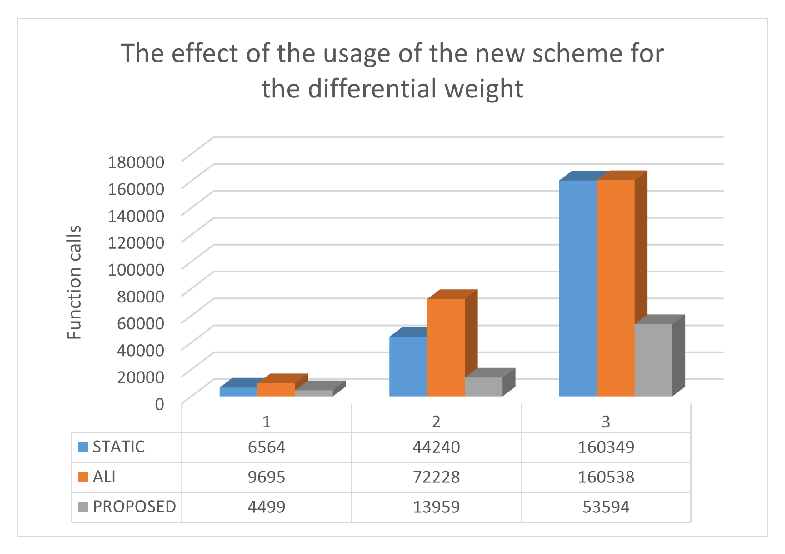
\includegraphics[scale=0.75]{image1}
\end{figure}
\begin{figure}
\caption{Plot of function calls using the two modifications.\label{fig:Plot2}}

\centering{}
\includegraphics[scale=0.75]{image2}
\end{figure}
\begin{figure}

\caption{Time comparisons for a variety of test functions.\label{fig:Time-comparisons-for}}

\centering{}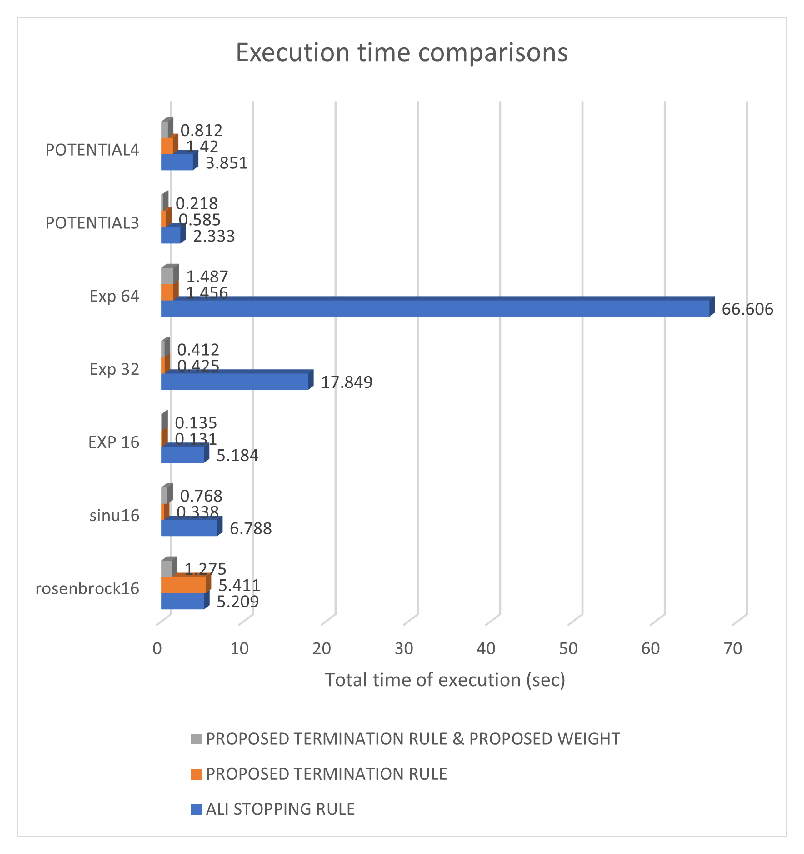
\includegraphics[scale=0.75]{time_comparison_de}
\end{figure}
\begin{figure}

\caption{Box plot representation and Wilcoxon rank-sum test results of the
comparison among the schemes for the differential weight. The stopping
rule used is the proposed by Ali in equation \ref{eq:termination_ali}.
A p-value of less than 0.05 (2-tailed) was used for statistical significance
and has been marked with bold.\label{fig:stat1}}

\centering{}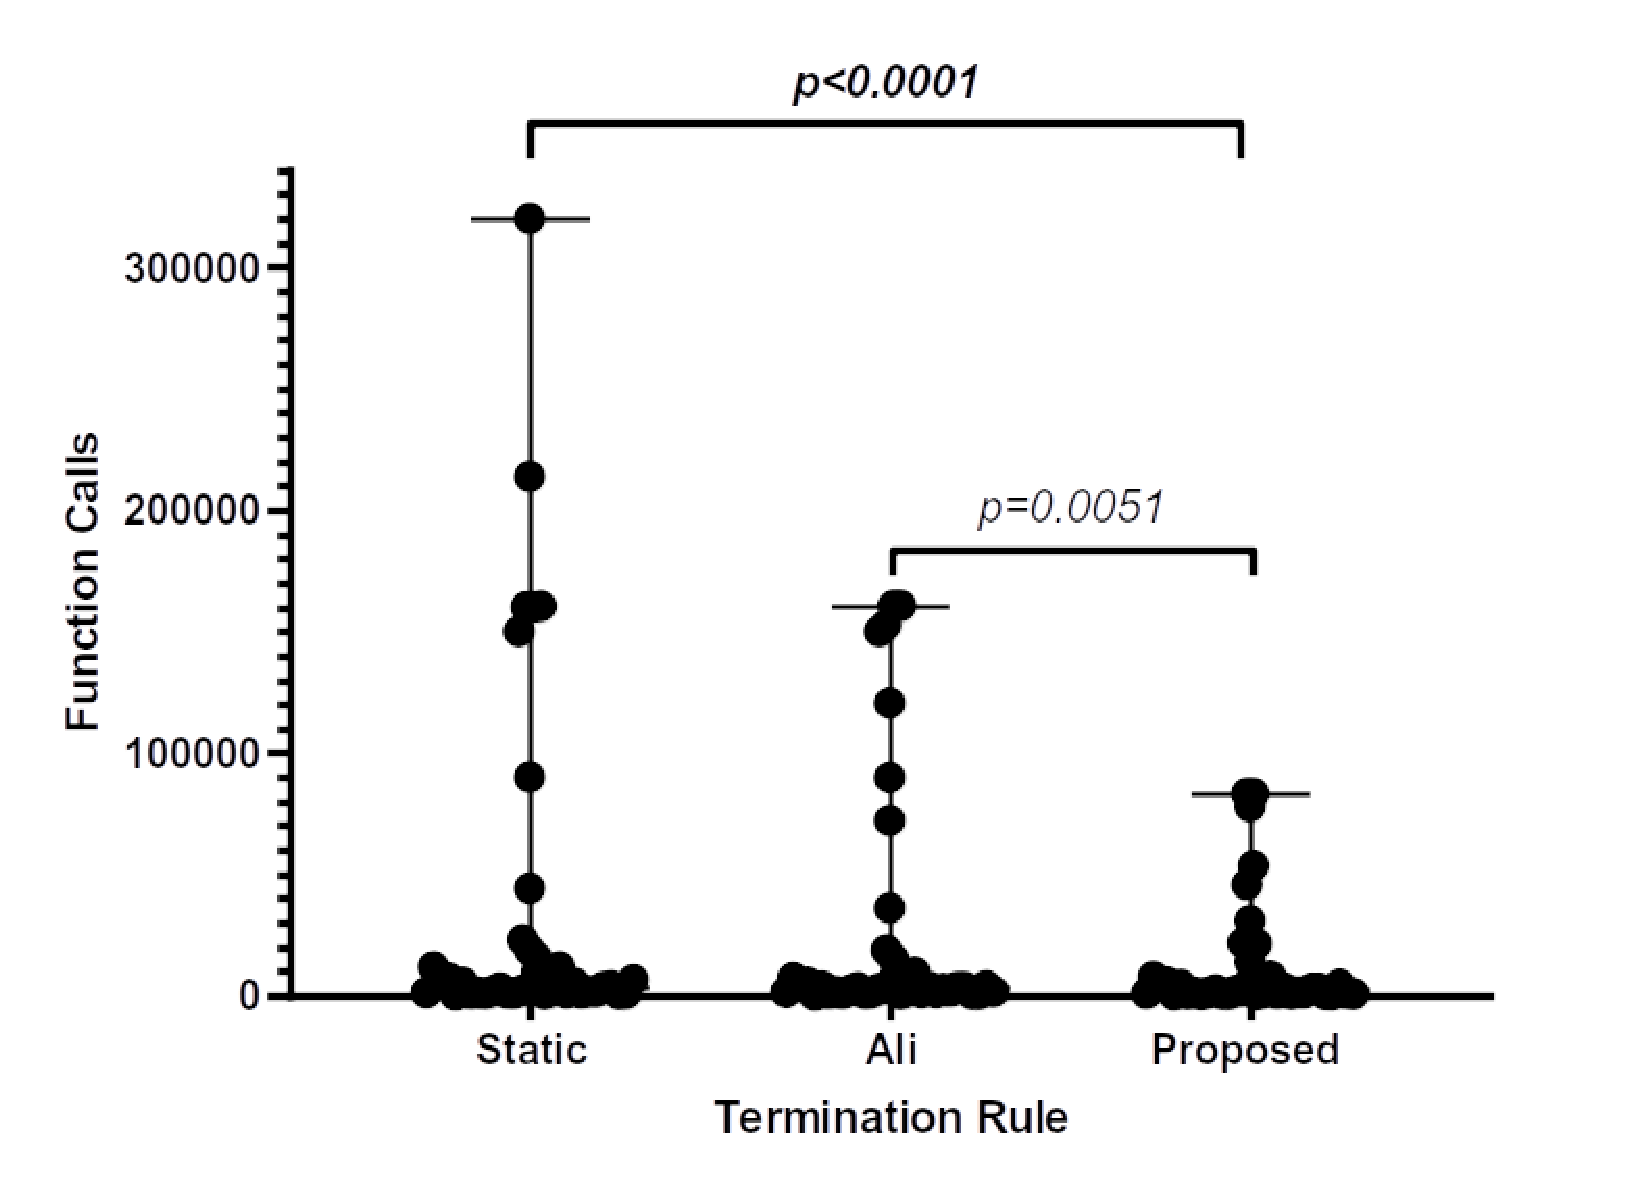
\includegraphics[scale=0.45]{stat_de}
\end{figure}


\section{Conclusions\label{sec:Conclusions}}

In this text, two main additions to the DE method are presented. In
the first an asymptotic termination rule was introduced and used successfully
even in multidimensional problems. This rule is based on the observation
that from one point onwards the average of the functional values of
the agents does not change. This means that either the algorithm has
already found the global minimum or its further continuation will
have no meaning. 

In the second case, a stochastic scheme was used to produce the differential
weight. This scheme helped the algorithm to better explore the search
space of the objective function without the need for more calls to
the objective function. 

The proposed modifications significantly speed up the original method
in terms of function calls in most cases. Each of the proposed modifications
can be used separately or together in the DE method. If used together
there is a large reduction in the number of required function calls
that reaches up to 80\% without problems in the reliability of the
method and its ability to successfully find the total minimum. 

The DE method can also be used in cases of optimization problems with
constraints as long as there is a change in the original problem so
that the constraints are included in the function with the usage for
example Langrage multipliers.

\subsection*{Compliance with Ethical Standards }

All authors declare that they have no has no conflict of interest. 

\subsection*{Acknowledgments}

The experiments of this research work was performed at the high performance
computing system established at Knowledge and Intelligent Computing
Laboratory, Dept of Informatics and Telecommunications, University
of Ioannina, acquired with the project \textquotedbl Educational
Laboratory equipment of TEI of Epirus\textquotedbl{} with MIS 5007094
funded by the Operational Programme \textquotedbl Epirus\textquotedbl{}
2014-2020, by ERDF and national finds.
\begin{thebibliography}{10}
\bibitem{go_physics1}Z.A. Kudyshev, A.V. Kildishev, V.M. Shalaev
and A. Boltasseva, Machine learning--assisted global optimization
of photonic devices, Nanophotonics \textbf{10}, pp. 371-383, 2021.

\bibitem{go_physics2}X.L. Ding, Z.Y. Li, J.H. Meng, Y.X. Zhao and
G.H. Sheng, Density-functional global optimization of $\left(\mbox{LA}_{2}\mbox{O}_{3}\right)_{n}$
clusters , J. Chem. Phys. \textbf{137}, 2012.

\bibitem{go_physics3}S. Morita and N. Naoki, Global optimization
of tensor renormalization group using the corner transfer matrix,
Phys. Rev. B \textbf{103}, 2021.

\bibitem{go_physics4}S. Heiles and R.L. Johnston, Global optimization
of clusters using electronic structure methods, Int. J. Quantum Chem.
\textbf{113}, pp. 2091-2109, 2013.

\bibitem{go_chem1}Y. Yang, T. Pan and J. Zhang, Global Optimization
of Norris Derivative Filtering with Application for Near-Infrared
Analysis of Serum Urea Nitrogen, American Journal of Analytical Chemistry
\textbf{10}, pp. 143-152, 2019.

\bibitem{go_chem2}C. Grebner, J. Becker, D. Weber and B. Engels,
Tabu search based global optimization algorithms for problems in computational
chemistry, J Cheminform \textbf{4}, pp. 10, 2012.

\bibitem{go_chem3}M. Dittner, J. M�ller, H.M. Aktulga and B.J. Hartke,
Efficient global optimization of reactive force-field parameters,
Comput. Chem. \textbf{36}, pp. 1550--1561, 2015.

\bibitem{go_econ1}W. Zhao, L. Wang and Z. Zhang, Supply-Demand-Based
Optimization: A Novel Economics-Inspired Algorithm for Global Optimization,
IEEE Access \textbf{7}, pp. 73182-73206, 2019.

\bibitem{go_econ2}S.K. Mishra, Global Optimization of Some Difficult
Benchmark Functions by Host-Parasite Co-Evolutionary Algorithm, Economics
Bulletin \textbf{33}, pp. 1-18, 2013.

\bibitem{key-16}H.A. Bremermann, A method for unconstrained global
optimization, Mathematical Biosciences \textbf{9}, pp. 1-15, 1970.

\bibitem{key-17}R.A. Jarvis, Adaptive global search by the process
of competitive evolution, IEEE Trans. on Syst., Man and Cybergenetics
\textbf{75}, pp. 297-311, 1975.

\bibitem{key-18}W.L. Price, Global Optimization by Controlled Random
Search, Computer Journal \textbf{20}, pp. 367-370, 1977.

\bibitem{key-19}S. Kirkpatrick, C.D. Gelatt, M.P. Vecchi, Optimization
by simulated annealing, Science \textbf{220}, pp. 671-680, 1983.

\bibitem{key-20}P. J. M. van Laarhoven, E. H. L. Aarts, Simulated
Annealing: Theory and Applications, 1987, D. Riedel, Boston.

\bibitem{key-21-1}A. Corana, M. Marchesi, C. Martini, S. Ridella,
Minimizing Multimodal Functions of Continuous Variables with the Simulated
Annealing Algorithm, ACM Transactions on Mathematical Software \textbf{13},
pp. 262-280, 1987.

\bibitem{key-22}W.L. Goffe, G.D. Ferrier, J. Rogers, Global Optimization
of Statistical Functions with Simulated Annealing, J. Econometrics
\textbf{60}, pp. 65-100, 1994.

\bibitem{key-23}D. Goldberg, Genetic Algorithms in Search, Optimization
and Machine Learning, Addison-Wesley Publishing Company, Reading,
Massachussets, 1989.

\bibitem{key-6}Z. Michaelewicz, Genetic Algorithms + Data Structures
= Evolution Programs. Springer - Verlag, Berlin, 1996.

\bibitem{bee1}B. Akay and D. Karaboga, A modified Artificial Bee
Colony algorithm for real-parameter optimization, Information Sciences
\textbf{192}, pp. 120-142, 2012.

\bibitem{bee2}G. Zhu and S. Kwong, Gbest-guided artificial bee colony
algorithm for numerical function optimization, Applied Mathematics
and Computation \textbf{217}, pp. 3166-3173, 2010.

\bibitem{aco}M. Dorigo, M. Birattari and T. Stutzle, Ant colony optimization,
IEEE Computational Intelligence Magazine \textbf{1}, pp. 28-39, 2006.

\bibitem{key-24}R. Storn, K. Price, Differential Evolution - A Simple
and Efficient Heuristic for Global Optimization over Continuous Spaces,
Journal of Global Optimization \textbf{11}, pp. 341-359, 1997.

\bibitem{key-25}J. Kennedy, R.C. Everhart, Particle Swarm Optimization.
In Proceedings of the 1995 IEEE International Conference on Neural
Networks, Vol. 4, pp. 1942-1948, IEEE Press, 1995.

\bibitem{de_main_paper}R. Storn, On the usage of differential evolution
for function optimization, In: Proceedings of North American Fuzzy
Information Processing, pp. 519-523, 1996.

\bibitem{gpu1}Y. Zhou and Y. Tan, GPU-based parallel particle swarm
optimization, In: 2009 IEEE Congress on Evolutionary Computation,
pp. 1493-1500, 2009.

\bibitem{gpu2}L. Dawson and I. Stewart, Improving Ant Colony Optimization
performance on the GPU using CUDA, In: 2013 IEEE Congress on Evolutionary
Computation, pp. 1901-1908, 2013.

\bibitem{gpu3}Barkalov, K., Gergel, V. Parallel global optimization
on GPU, J Glob Optim \textbf{66}, pp. 3--20, 2016.

\bibitem{de_review1}Z. Wu, N. Cui, L. Zhao, L. Han, X. Hu, H. Cai,
D. Gong, L.�Xing, X. Chen, B.�Zhu, M.�lv, S.�Zhu, Q.�Liu, Estimation
of maize evapotranspiration in semi-humid regions of Northern China
Using Penman-Monteith model and segmentally optimized Jarvis model,
Journal of Hydrology \textbf{22}, pp 127483, 2022.

\bibitem{de_review2}E. Tlelo-Cuautle,� A.M. Gonz�lez-Zapata,� J.D.
D�az-Mu�oz,� L.G. de la Fraga�and I. Cruz-Vega, Optimization of fractional-order
chaotic cellular neural networks by metaheuristics, The European Physical
Journal Special Topics, 2022.

\bibitem{de_review3}G. Sun,�C. Li�and�L. Deng, An adaptive regeneration
framework based on search space adjustment for differential evolution,
Neural Computing and Applications�\textbf{33},�pp. 9503--9519, 2021

\bibitem{de_review4}P. Civiciogluan and E. Besdok, Bernstain-search
differential evolution algorithm for numerical function optimization,
Expert Systems with Applications \textbf{138}, 2019.

\bibitem{de_review6}J. Liang, K. Qiao, K. Yu, S.Ge ,B. Qu, R. Xu
and K. Li, Parameters estimation of solar photovoltaic models via
a self-adaptive ensemble-based differential evolution, Solar Energy
\textbf{207}, pp. 336-346, 2020.

\bibitem{de_review7}L. Peng, S. Liu, R. Liu and Lin Wang, Effective
long short-term memory with differential evolution algorithm for electricity
price prediction, Energy \textbf{162}, pp. 1301-1314, 2018.

\bibitem{de_review8}N. Awad and N. Mallik and F. Hutter, Differential
Evolution for Neural Architecture Search, In Proceedings of the 1st
workshop on neural architecture search, 2020.

\bibitem{de_neural1}J. Ilonen, J.K. Kamarainen and J. Lampinen, Differential
Evolution Training Algorithm for Feed-Forward Neural Networks, Neural
Processing Letters \textbf{17}, pp. 93--105, 2003.

\bibitem{de_neural2}A. Slowik, Application of an Adaptive Differential
Evolution Algorithm With Multiple Trial Vectors to Artificial Neural
Network Training, IEEE Transactions on Industrial Electronics \textbf{58},
pp. 3160-3167, 2011.

\bibitem{de_neural3}L. Wang, Y. Zeng and T. Chen, Back propagation
neural network with adaptive differential evolution algorithm for
time series forecasting, Expert Systems with Applications \textbf{42},
pp. 855-863, 2015.

\bibitem{de_tsp}X. Wang, G. Xu, Hybrid Differential Evolution Algorithm
for Traveling Salesman Problem, Procedia Engineering \textbf{15},
pp. 2716-2720, 2011.

\bibitem{de_review5}I.M.Ali , D. Essam and K. Kasmarik, A novel design
of differential evolution for solving discrete traveling salesman
problems, Swarm and Evolutionary Computation \textbf{52}, 2020.

\bibitem{rbf_de1}J. Liu and J. Lampinen, A differential evolution
based incremental training method for RBF networks, In Proceedings
of the 7th annual conference on Genetic and evolutionary computation
(GECCO '05), pp. 881--888, 2005.

\bibitem{rbf_de2}B. O'Hora, J. Perera and A. Brabazon, Designing
Radial Basis Function Networks for Classification Using Differential
Evolution, In: The 2006 IEEE International Joint Conference on Neural
Network Proceedings, pp. 2932-2937, 2006.

\bibitem{rbf_de3}N. Naveen , V. Ravi , C. Raghavendra Rao and N.
Chauhan, Differential evolution trained radial basis function network:
application to bankruptcy prediction in banks, International Journal
of Bio-Inspired Computation \textbf{2}, pp. 222-232, 2010.

\bibitem{lennardjones_de1}Z. Chen, X. Jiang, J. Li, S. Li and L.
Wang, PDECO: Parallel differential evolution for clusters optimization,
J. Comput. Chem. \textbf{34}, pp. 1046-1059. 2013.

\bibitem{lennardjones_de2}A. Ghosh, R. Mallipeddi, S. Das and A.
K. Das, A Switched Parameter Differential Evolution with Multi-donor
Mutation and Annealing Based Local Search for Optimization of Lennard-Jones
Atomic Clusters, In: 2018 IEEE Congress on Evolutionary Computation
(CEC), pp. 1-8, 2018.

\bibitem{compact_de}E. Mininno, F. Neri, F. Cupertino and D. Naso,
Compact Differential Evolution, IEEE Transactions on Evolutionary
Computation \textbf{15}, pp. 32-54, 2011.

\bibitem{self_de}A. K. Qin, V. L. Huang and P. N. Suganthan, Differential
Evolution Algorithm With Strategy Adaptation for Global Numerical
Optimization, IEEE Transactions on Evolutionary Computation \textbf{13},
pp. 398-417, 2009.

\bibitem{fuzzy_de}J. Liu, J. Lampinen, A Fuzzy Adaptive Differential
Evolution Algorithm, Soft Comput \textbf{9}, pp. 448--462, 2005. 

\bibitem{parellel_de}H. Wang, S. Rahnamayan and Z. Wu, Parallel differential
evolution with self-adapting control parameters and generalized opposition-based
learning for solving high-dimensional optimization problems, Journal
of Parallel and Distributed Computing \textbf{73}, pp. 62-73, 2013.

\bibitem{survey_de}S. Das, S.S. Mullick and P.N. Suganthan, Recent
advances in differential evolution -- An updated survey, Swarm and
Evolutionary Computation \textbf{27}, pp. 1-30, 2016.

\bibitem{ali_de}M.M. Ali and A. T�rn, Population set-based global
optimization algorithms: some modifications and numerical studies,
Computers \& Operations Research \textbf{31}, pp. 1703-1725, 2004.

\bibitem{Ali1}M. Montaz Ali, Charoenchai Khompatraporn, Zelda B.
Zabinsky, A Numerical Evaluation of Several Stochastic Algorithms
on Selected Continuous Global Optimization Test Problems, Journal
of Global Optimization \textbf{31}, pp 635-672, 2005. 

\bibitem{Floudas1}C.A. Floudas, P.M. Pardalos, C. Adjiman, W. Esposoto,
Z. G$\ddot{\mbox{u}}$m$\ddot{\mbox{u}}$s, S. Harding, J. Klepeis,
C. Meyer, C. Schweiger, Handbook of Test Problems in Local and Global
Optimization, Kluwer Academic Publishers, Dordrecht, 1999.

\bibitem{testfunctions1}M.M. Ali and P. Kaelo, Improved particle
swarm algorithms for global optimization, Applied Mathematics and
Computation \textbf{196}, pp. 578-593, 2008.

\bibitem{testfunctions2}H. Koyuncu, R. Ceylan, A PSO based approach:
Scout particle swarm algorithm for continuous global optimization
problems, Journal of Computational Design and Engineering \textbf{6},
pp. 129--142, 2019.

\bibitem{testfunctions3}Patrick Siarry, G�rard Berthiau, Fran�ois
Durdin, Jacques Haussy, ACM Transactions on Mathematical Software
\textbf{23}, pp 209--228, 1997.

\bibitem{testfunctions4}I.G. Tsoulos, I.E. Lagaris, GenMin: An enhanced
genetic algorithm for global optimization, Computer Physics Communications\textbf{
178, }pp. 843-851, 2008.

\bibitem{Powell}M.J.D Powell, A Tolerant Algorithm for Linearly Constrained
Optimization Calculations, Mathematical Programming \textbf{45}, pp.
547-566, 1989. 

\bibitem{gkls}M. Gaviano, D.E. Ksasov, D. Lera, Y.D. Sergeyev, Software
for generation of classes of test functions with known local and global
minima for global optimization, ACM Trans. Math. Softw. \textbf{29},
pp. 469-480, 2003.

\bibitem{Jones}J.E. Lennard-Jones, On the Determination of Molecular
Fields, Proc. R. Soc. Lond. A \textbf{ 106}, pp. 463--477, 1924.
\end{thebibliography}

\end{document}
